\documentclass[aspectratio=169]{beamer}
\usetheme{Boadilla}

% ---------------------------------------------------------
% Premium Academic Color Theme (Slate Blue & Crimson Accents)
% ---------------------------------------------------------
\definecolor{navyblue}{RGB}{20, 54, 95}
\definecolor{crimsonred}{RGB}{141, 8, 28}
\definecolor{charcoal}{RGB}{43, 43, 43}
\definecolor{lightgray}{RGB}{245, 245, 245}

\usecolortheme[named=navyblue]{structure}
\setbeamercolor{title}{bg=navyblue, fg=white}
\setbeamercolor{frametitle}{bg=navyblue, fg=white}
\setbeamercolor{block title}{bg=navyblue, fg=white}
\setbeamercolor{block body}{bg=lightgray, fg=charcoal}
\setbeamercolor{block title alerted}{bg=crimsonred, fg=white}
\setbeamercolor{block body alerted}{bg=lightgray, fg=charcoal}

\setbeamertemplate{navigation symbols}{} % Hide default navigation icons
\setbeamertemplate{headline}{}

% Packages
\usepackage[utf8]{inputenc}
\usepackage{graphicx}
\usepackage{booktabs}
\usepackage{amsmath}
\usepackage{amssymb}
\usepackage{listings}
\usepackage{hyperref}

% Code snippet styles
\lstset{
    language=Python,
    basicstyle=\ttfamily\tiny,
    keywordstyle=\color{navyblue}\bfseries,
    commentstyle=\color{gray}\itshape,
    stringstyle=\color{crimsonred},
    showstringspaces=false,
    breaklines=true,
    backgroundcolor=\color{lightgray},
    frame=single,
    rulecolor=\color{lightgray}
}

% ---------------------------------------------------------
% Presentation Details
% ---------------------------------------------------------
\title[AMPT Course — Day 1]{Day 1: Foundations of Relativistic Kinematics \& Experimental HEP}
\subtitle{14-Day Hands-on Course on Heavy-Ion Phenomenology}
\author[MSc-Lecture Series]{ Lecture }
\institute[HEP Group]{NIT-J,HEP-119}
\date{June 2026}

\begin{document}

% Slide 1: Title Slide
\begin{frame}
    \titlepage
\end{frame}

% Slide 2: 14-Day Course Syllabus Overview
\begin{frame}{Syllabus: 14-Day Hands-on Course Layout}
    \begin{columns}
        \begin{column}{0.5\textwidth}
            \footnotesize
            \textbf{Part I: Relativistic Kinematics}
            \begin{itemize}
                \item \textbf{Day 1: Experimental HEP, Boosts \& Rapidity}
                \item Day 2: Kinematics I: 4-vectors \& CMS energy
                \item Day 3: Kinematics II: Rapidity \& Pseudorapidity
                \item Day 4: Kinematics III: Invariant Yield \& Phase Space
            \end{itemize}
            \vspace{0.05cm}
            \textbf{Part II: AMPT Physics \& Mechanics}
            \begin{itemize}
                \item Day 5: AMPT Evolution: HIJING, ZPC, Hadronization, ART
                \item Day 6: AMPT Data format: event headers \& parsing
                \item Day 7: Single-Particle Observables: Multiplicity \& $p_T$
            \end{itemize}
        \end{column}
        \begin{column}{0.5\textwidth}
            \footnotesize
            \textbf{Part III: Thermodynamics \& Collectivity}
            \begin{itemize}
                \item Day 8: Transverse Spectra, Identified Particles \& $m_T$ Scaling
                \item Day 9: Centrality \& Geometry: Glauber vs AMPT
                \item Day 10: Collective Flow: Elliptic Flow ($v_2$)
                \item Day 11: Medium Modification: ZPC Knobs \& Mean Free Path
            \end{itemize}
            \vspace{0.1cm}
            \textbf{Part IV: Advanced Scans \& Pipeline}
            \begin{itemize}
                \item Day 12: Energy Scan: Beam Energy Scan (STAR at RHIC)
                \item Day 13: Advanced Analysis
                \item Day 14: Wrap-Up: Reproducible HEP Data Pipeline
            \end{itemize}
        \end{column}
    \end{columns}
\end{frame}

\section{Detector Physics}

% Slide 3: Why Experimental HEP: Probing the Extremes
\begin{frame}{Why Experimental High Energy Physics? Probing the Extremes}
    \begin{block}{The QGP Phase \& Early Universe}
        \begin{itemize}
            \item We collide heavy nuclei at ultra-relativistic velocities to recreate the conditions of the early universe ($10^{-6}$ seconds after the Big Bang).
            \item **The Quark-Gluon Plasma (QGP):** A state of deconfined, color-charged quarks and gluons.
        \end{itemize}
    \end{block}
    \begin{block}{The QCD Confinement Challenge}
        \begin{itemize}
            \item Hadrons are held together by strong force (QCD). Because of color confinement, we cannot isolate individual quarks/gluons directly.
            \item **Solution:** We must analyze final-state hadron sprays to infer the plasma's thermodynamic and transport properties.
        \end{itemize}
    \end{block}
\end{frame}

% Slide 4: Collision Energetics: Why Accelerators?
\begin{frame}{Collision Energetics: Why Accelerators?}
    \begin{block}{Resolving Matter at Sub-Femtometer Scales}
        \begin{itemize}
            \item Accelerators provide high center-of-mass energies ($\sqrt{s}$) to satisfy mass-energy equivalence ($E=mc^2$).
            \item Short de Broglie wavelengths probe smaller structures: $\lambda = h/p$.
        \end{itemize}
    \end{block}
    \begin{alertblock}{Interactive Physics Simulator}
        Open in your browser:
        \begin{itemize}
            \item \texttt{animations/03\_debroglie\_resolution\_probing.html} \quad {\tiny (de Broglie wave probe, Airy disk resolution, \& sub-nuclear scale probing)}
        \end{itemize}
    \end{alertblock}
\end{frame}

% Slide 5: Center-of-Mass Energy Mappings
\begin{frame}{Center-of-Mass Energy Mappings}
    \begin{block}{Center-of-Mass Energy Formulas}
        \begin{itemize}
            \item **Collider Advantage:** In a collider ($E_{\text{beam1}} = E_{\text{beam2}} = E$), center-of-mass energy scales linearly:
            \[ \sqrt{s_{\text{collider}}} \approx 2E \]
            \item **Fixed Target Limit:** In a fixed-target collision (beam energy $E$ on target nucleon mass $m_N$), energy scales only as the square root:
            \[ \sqrt{s_{\text{fixed}}} \approx \sqrt{2 m_N E} \]
        \end{itemize}
    \end{block}
    \begin{block}{Kinematic Consequence of Fixed-Target Scaling}
        To match the LHC center-of-mass energy of $\sqrt{s} = 13.6$ TeV in a fixed-target collision (beam energy $E$ on stationary proton mass $m_p \approx 1$ GeV):
        \[ E_{\text{beam}} = \frac{s}{2m_p} \approx \frac{185 \text{ TeV}^2}{2 \text{ GeV}} \approx 92,500 \text{ GeV} = 92.5 \text{ TeV} \]
        This astronomical engineering requirement proves why colliders are indispensable for high-energy QGP searches!
    \end{block}
\end{frame}

% Slide 6: Fixed-Target vs. Collider Geometry (Energetics comparison)
\begin{frame}{Fixed-Target vs. Collider Geometry}
    \begin{block}{Center-of-Mass Energetics Comparison}
        Let us calculate the beam energy required to match LHC and RHIC center-of-mass energies in a fixed-target configuration:
    \end{block}
    \begin{table}
        \centering
        \footnotesize
        \begin{tabular}{lccr}
            \toprule
            \textbf{System} & \textbf{Collider $\sqrt{s_{NN}}$} & \textbf{Fixed-Target Equivalent $E_{\text{beam}}$} & \textbf{Kinematic Advantage} \\
            \midrule
            SPS ($p+p$) & $17.3$ GeV & $158$ GeV & Baseline \\
            RHIC ($Au+Au$) & $200$ GeV & $21.3$ TeV & $100 \times$ Beam boost \\
            LHC ($Pb+Pb$) & $5.02$ TeV & $13.5$ PeV (13,500 TeV) & Outside classical accelerator tech \\
            \bottomrule
        \end{tabular}
    \end{table}
    \begin{alertblock}{Interactive Simulation}
        Open our custom simulator at \texttt{animations/collision\_animation.html} to interactively run collisions and observe the center-of-mass energy transformations.
    \end{alertblock}
\end{frame}

% Slide 6: Specialization by Design: Belle II vs. LHCb
\begin{frame}{Specialization by Design: Belle II vs. LHCb}
    \begin{columns}
        \begin{column}{0.5\textwidth}
            \begin{block}{Belle II (KEKB Asymmetric Collider)}
                \begin{itemize}
                    \item **Beams:** $8.0$ GeV $e^-$ on $3.5$ GeV $e^+$.
                    \item **Design:** Collides asymmetric energies to provide a longitudinal Lorentz boost to the center of mass.
                    \item **Physics:** Allows precise decay-length measurements of short-lived B-mesons ($B \rightarrow J/\psi K_S^0$) to study CP violation.
                \end{itemize}
            \end{block}
        \end{column}
        \begin{column}{0.5\textwidth}
            \begin{block}{LHCb (LHC Forward Spectrometer)}
                \begin{itemize}
                    \item **Beams:** Symmetric proton-proton at 13.6 TeV.
                    \item **Design:** Forward single-arm cone spectrometer ($2 < \eta < 5$).
                    \item **Physics:** At LHC energies, $b\bar{b}$ pairs are produced at very forward/backward angles. Placed in the forward direction to capture these heavy flavor hadrons.
                \end{itemize}
            \end{block}
        \end{column}
    \end{columns}
\end{frame}

% Slide 7: Specialization by Design: STAR vs. CMS vs. ALICE
\begin{frame}{Specialization by Design: STAR vs. CMS vs. ALICE}
    \begin{columns}
        \begin{column}{0.33\textwidth}
            \begin{block}{ALICE (LHC)}
                \tiny
                \textbf{QGP Specialized Tracking}
                \begin{itemize}
                    \item Optimized for extreme track density ($Pb+Pb$ collisions).
                    \item Extremely low material budget and magnetic field ($0.5$ T) to track and identify very low-$p_T$ hadrons.
                \end{itemize}
            \end{block}
        \end{column}
        \begin{column}{0.33\textwidth}
            \begin{block}{STAR (RHIC)}
                \tiny
                \textbf{Hadron Spectroscopy}
                \begin{itemize}
                    \item Massive Time Projection Chamber (TPC) optimized for particle identification, centrality scans, and collective flow physics at RHIC energies.
                \end{itemize}
            \end{block}
        \end{column}
        \begin{column}{0.33\textwidth}
            \begin{block}{CMS (LHC)}
                \tiny
                \textbf{High-$p_T$ \& High-Luminosity}
                \begin{itemize}
                    \item Built around a massive $3.8$ T superconducting solenoid.
                    \item High-granularity silicon trackers and deep EM/Hadronic calorimeters designed to capture high-$p_T$ jets, leptons, and Higgs candidates.
                \end{itemize}
            \end{block}
        \end{column}
    \end{columns}
\end{frame}

% Slide 8: Layered "Onion" Detector Architecture
\begin{frame}{Layered "Onion" Detector Architecture}
    \begin{block}{Concentric Cylindrical Configurations}
        To track and reconstruct every single final-state particle, modern cylindrical colliders use concentric detector layers centered around the beam axis:
    \end{block}
    \begin{enumerate}
        \item **Vertex Detectors (Inner Silicon):** Capture prompt secondary decays close to the interaction point.
        \item **Central Trackers (TPC / Drift Chambers):** Map trajectories under magnetic fields to resolve momenta.
        \item **Particle Identification (TOF / RICH):** Separate pions, kaons, and protons.
        \item **Electromagnetic Calorimeters (EMCal):** Capture electron and photon energy.
        \item **Hadronic Calorimeters (HCal):** Absorb hadronic shower energy.
        \item **Muon Spectrometer:** Outermost chambers that capture highly penetrating muons.
    \end{enumerate}
\end{frame}

% Slide 9: Tracking & Curvature in Time Projection Chambers (TPC)
\begin{frame}{Tracking \& Curvature in Time Projection Chambers (TPC)}
    \begin{columns}
        \begin{column}{0.5\textwidth}
            \begin{block}{TPC Operation Principles}
                \begin{itemize}
                    \item Gas-filled drift chamber placed inside high electric and magnetic fields.
                    \item Traversing charged particles ionize gas atoms, producing electrons that drift towards anodes.
                    \item Reconstructs 3D tracks from anode pixels ($X,Y$) and drift times ($Z$).
                \end{itemize}
            \end{block}
        \end{column}
        \begin{column}{0.5\textwidth}
            \begin{block}{TPC Physics Outputs}
                \begin{itemize}
                    \item **Momentum Measurement:** Curved tracks in magnetic field $B$ yield momentum $p$:
                    \[ p = 0.3 \cdot B \cdot R \]
                    where $R$ is the curvature radius.
                    \item **Energy Loss ($dE/dx$):** Measures the rate of specific ionization loss to identify particles via Bethe-Bloch curves at low momentum.
                \end{itemize}
            \end{block}
        \end{column}
    \end{columns}
\end{frame}

% Slide 10: Particle Identification (PID): Time-of-Flight vs. RICH
\begin{frame}{Particle Identification (PID): Time-of-Flight vs. RICH}
    \begin{columns}
        \begin{column}{0.5\textwidth}
            \begin{block}{Time-of-Flight (TOF) Systems}
                \begin{itemize}
                    \item Measures the time difference $\Delta t$ between collision vertex and detector impact.
                    \item **TOF Resolution:** High-precision Multigap Resistive Plate Chambers (MRPC) achieve resolutions of $\sigma_t \sim 50\text{--}80$ ps.
                    \item Separates pions, kaons, and protons at low-intermediate transverse momenta.
                \end{itemize}
            \end{block}
        \end{column}
        \begin{column}{0.5\textwidth}
            \begin{block}{Ring Imaging Cherenkov (RICH)}
                \begin{itemize}
                    \item Relies on Cherenkov radiation emitted when a particle's speed exceeds speed of light in medium: $\beta > 1/n$.
                    \item Measures Cherenkov angle $\theta_C$:
                    \[ \cos\theta_C = \frac{1}{n\beta} \]
                    \item Projects rings onto photon detectors, separating high-momentum species.
                \end{itemize}
            \end{block}
        \end{column}
    \end{columns}
\end{frame}

% Slide 11: Energy Capture: Calorimeters & Muon Spectrometers
\begin{frame}{Energy Capture: Calorimeters \& Muon Spectrometers}
    \begin{columns}
        \begin{column}{0.5\textwidth}
            \begin{block}{Calorimetry Layers}
                \begin{itemize}
                    \item **Electromagnetic Calorimeter (EMCal):** Uses high-Z absorbers (e.g. Lead-Tungstate crystals) to trigger Bremsstrahlung showers, capturing all $e^\pm$ and $\gamma$ energy.
                    \item **Hadronic Calorimeter (HCal):** Absorbs strongly interacting hadrons ($\pi^\pm, K^\pm, p, n$) through inelastic nuclear interactions.
                \end{itemize}
            \end{block}
        \end{column}
        \begin{column}{0.5\textwidth}
            \begin{block}{Muon Spectrometers}
                \begin{itemize}
                    \item Muons are minimum ionizing particles (MIPs) and do not trigger hadronic or electromagnetic showers.
                    \item They penetrate through thick iron shielding.
                    \item Placed outermost to record clean muon tracks (crucial for vector meson decay $J/\psi \rightarrow \mu^+\mu^-$).
                \end{itemize}
            \end{block}
        \end{column}
    \end{columns}
\end{frame}

\section{Why AMPT?}

% Slide 12: Why AMPT? The Dynamical Multi-Phase Transport
\begin{frame}{Why AMPT? The Dynamical Multi-Phase Transport}
    \begin{block}{The Physics Motivation}
        \begin{itemize}
            \item Detectors only record the asymptotic hadronic state after **kinetic freeze-out**.
            \item **AMPT (A Multi-Phase Transport)** is a dynamical Monte Carlo transport model that reconstructs the complete collision history:
            \[ \text{Initial Geometry (HIJING)} \rightarrow \text{Parton Cascade (ZPC)} \rightarrow \text{Hadronization (Coalescence)} \rightarrow \text{Hadron Transport (ART)} \]
        \end{itemize}
    \end{block}
    \begin{block}{Course Outcomes for Students}
        By the end of this 14-day course, you will be able to:
        \begin{enumerate}
            \item Stream and parse raw simulated heavy-ion data.
            \item Code relativistic kinematics and flow observables ($v_2$) from scratch.
            \item Build full reproducible data analysis pipelines.
        \end{enumerate}
    \end{block}
\end{frame}

\section{Relativistic Boosts}

% Slide 13: Relativistic Boosts: Successive Collinear Boosts
\begin{frame}{Relativistic Kinematics: Collinear Boosts (Sahoo pg. 115-116)}
    \begin{block}{Successive Boosts along X-axis}
        Consider three collinear inertial frames of reference $S \xrightarrow{v} S' \xrightarrow{u} S''$ moving along the positive X-axis (Sahoo Fig. 5.6):
    \end{block}
    \begin{columns}
        \begin{column}{0.5\textwidth}
            \footnotesize
            **Boost 1: $S \rightarrow S'$ with velocity $v$ ($\beta_1 = v/c$):**
            \[ x'^{0} = \gamma_v (x^0 - \beta_1 x^1) \]
            \[ x'^{1} = \gamma_v (x^1 - \beta_1 x^0) \]
            where $\gamma_v = \frac{1}{\sqrt{1 - \beta_1^2}}$
        \end{column}
        \begin{column}{0.5\textwidth}
            \footnotesize
            **Boost 2: $S' \rightarrow S''$ with velocity $u$ ($\beta_2 = u/c$):**
            \[ x''^{0} = \gamma_u (x'^{0} - \beta_2 x'^{1}) \]
            \[ x''^{1} = \gamma_u (x'^{1} - \beta_2 x'^{0}) \]
            where $\gamma_u = \frac{1}{\sqrt{1 - \beta_2^2}}$
        \end{column}
    \end{columns}
\end{frame}

% Slide 14: Relativistic Velocity Addition: Non-Linearity & Speed Limit
\begin{frame}{Relativistic Velocity Addition}
    \begin{block}{Combined Single Boost $S \rightarrow S''$ with velocity $w$}
        Substituting the coordinate equations from Boost 1 into Boost 2 yields the effective relativistic velocity boost factor (Sahoo Eq. 5.41):
        \[ w = \frac{v + u}{1 + \frac{vu}{c^2}} \]
        And the total combined Lorentz factor becomes (Sahoo Eq. 5.39):
        \[ \gamma_w = \gamma_u \gamma_v \left( 1 + \frac{uv}{c^2} \right) \]
    \end{block}
    \begin{alertblock}{Interactive Relativistic Demonstrations}
        Open in your browser:
        \begin{itemize}
            \item \texttt{animations/rapidity\_boost.html} \quad {\tiny (Linear rapidity boosts \& additivity)}
            \item \texttt{animations/01\_velocity\_saturation\_comparison.html} \quad {\tiny (Validates \texttt{day01\_problem1})}
            \item \texttt{animations/02\_spacetime\_minkowski\_diagram.html} \quad {\tiny (Hyperbolic geometry visualized)}
        \end{itemize}
    \end{alertblock}
\end{frame}

% Slide 15: Rigorous Limits: Relativistic Saturation vs. Classical
\begin{frame}{Rigorous Limits of Velocity Addition}
    \begin{block}{Universal Speed Limit}
        This non-linearity guarantees that the speed of light $c$ is the absolute speed limit in the universe:
        \[ \text{If } v \rightarrow c \quad \text{or} \quad u \rightarrow c \quad \Rightarrow \quad w \rightarrow c \]
    \end{block}
    \begin{block}{Classical vs. Relativistic Velocity Saturation}
        In Problem 1 of the hands-on lab, you will successively add collinear boosts of $0.1c$ up to 20 times. 
        - **Classical sum** grows linearly to $2.0c$.
        - **Relativistic sum** saturates at $0.964c$, asymptotically approaching $1.0c$, as shown in your saved plot \texttt{day01\_problem1\_velocity\_rapidity.png}.
    \end{block}
\end{frame}

\section{Rapidity Additivity}

% Slide 16: Rapidity Definition: Hyperbolic Rotations in Spacetime
\begin{frame}{Rapidity Definition (Sahoo pg. 117-118)}
    \begin{block}{Hyperbolic Transformations in Minkowski Space}
        Because velocity addition is highly non-linear, measuring spectrum shapes and calculating transformations across moving frames in colliders is mathematically complex. We define a new hyperbolic angle called **Rapidity** ($y$):
        \[ y = \tanh^{-1}(\beta) = \frac{1}{2} \ln \left( \frac{1+\beta}{1-\beta} \right) \]
        Hyperbolic mappings transform the velocity parameter:
        \[ \beta = \tanh(y), \quad \gamma = \cosh(y), \quad \gamma\beta = \sinh(y) \]
    \end{block}
\end{frame}

% Slide 17: Proof of Rapidity Additivity
\begin{frame}{Proof of Rapidity Additivity: Mathematical Derivation}
    \begin{block}{Hyperbolic Angle Transformations (Sahoo pg. 117-118)}
        Let $y_1 = \tanh^{-1}(u/c)$ and $y_2 = \tanh^{-1}(v/c)$ represent two collinear boosts (taking $c=1$):
        \[ w = \frac{u+v}{1 + uv} = \frac{\tanh y_1 + \tanh y_2}{1 + \tanh y_1 \tanh y_2} \]
    \end{block}
    \begin{block}{The Hyperbolic Tangent Identity}
        Recalling the standard hyperbolic tangent angle-addition identity:
        \[ \tanh(y_1 + y_2) = \frac{\tanh y_1 + \tanh y_2}{1 + \tanh y_1 \tanh y_2} \]
        Which gives us the combined velocity parameter:
        \[ w = \tanh(y_1 + y_2) \]
    \end{block}
\end{frame}

% Slide 18: Rapidity Additivity: Physical Consequences
\begin{frame}{Rapidity Additivity: Physical Consequences}
    \begin{block}{Proving Linear Additivity (Sahoo Eq. 5.43)}
        Since the effective relativistic velocity boost is $w = \tanh(y_{\text{tot}})$, substituting our derivation yields:
        \[ \tanh(y_{\text{tot}}) = \tanh(y_1 + y_2) \quad \Rightarrow \quad y_{\text{tot}} = y_1 + y_2 \]
        This simple, elegant relation proves that collinear boosts combine linearly under rapidity!
    \end{block}
    \begin{alertblock}{Takeaway: Natural Collider Spectroscopy Variable}
        * **Velocity Addition** is highly non-linear, making cross-frame spectrum transformations mathematically complex.
        * **Rapidity Addition** is linear. Boosts along the beam axis simply shift the rapidity distribution by a constant ($y \rightarrow y + y_{\text{boost}}$), keeping the shape of the invariant yield distribution $dN/dy$ perfectly invariant!
    \end{alertblock}
\end{frame}

\section{CMS Kinematics}

% Slide 18: Kinematics in the Center-of-Momentum System (CMS)
\begin{frame}{Kinematics in the Center-of-Momentum System (Sahoo pg. 113-114)}
    \begin{block}{Asymmetric 2-Body Kinematics}
        Let $p_1$ and $p_2$ be the momentum 4-vectors of two colliding particles with masses $m_1$ and $m_2$. Let $P = p_1 + p_2$ be the total center-of-momentum 4-vector, with total invariant mass squared:
        \[ P^2 = (p_1 + p_2)^2 = M^2 = s \]
    \end{block}
    \begin{block}{Individual CMS Energies (Sahoo Eq. 5.29 \& 5.30)}
        Transforming to the center-of-momentum frame ($P = (\sqrt{s}, \vec{0})$) yields:
        \[ E_1^* = \frac{s + m_1^2 - m_2^2}{2\sqrt{s}} \]
        \[ E_2^* = \frac{s - m_1^2 + m_2^2}{2\sqrt{s}} \]
    \end{block}
\end{frame}

% Slide 19: CMS Momentum & Relative Velocity
\begin{frame}{CMS Momentum \& Relative Velocity}
    \begin{block}{CMS Momentum $p^*$ (Sahoo Eq. 5.32)}
        By using the invariant mass relation $E_1^{*2} - |\vec{p}^*|^2 = m_1^2$, we solve for the exact center-of-momentum three-momentum magnitude:
        \[ |\vec{p}^*|^2 = \frac{s^2 - 2s(m_1^2 + m_2^2) + (m_1^2 - m_2^2)^2}{4s} \]
        Note that $E_1^* + E_2^* = \sqrt{s}$ and the particles move in opposite directions with equal momentum magnitude: $\vec{p}_1^* = -\vec{p}_2^*$.
    \end{block}
    \begin{block}{Relative CMS Velocity (Sahoo Eq. 5.33)}
        The relative CMS velocity parameter is calculated as:
        \[ v_{12}^* = \left( \frac{|\vec{p}^*|}{E_1^*} \right)^2 \]
    \end{block}
\end{frame}

% Slide 20: Real Data: Symmetric vs. Asymmetric CMS Kinematics
\begin{frame}{Real Data: Symmetric vs. Asymmetric CMS Kinematics}
    \begin{block}{Computed Metrics from Problem 2}
        These exact kinematic formulas yield the following physical values for symmetric and asymmetric collider configurations:
    \end{block}
    \begin{itemize}
        \item **Symmetric $p+p$ at ALICE ($\sqrt{s} = 13.6$ TeV):**
        \[ E_1^* = E_2^* = 6800.000\text{ GeV}, \quad p^* = 6800.000\text{ GeV/c} \]
        \item **Symmetric $Au+Au$ at STAR ($\sqrt{s_{NN}} = 200$ GeV):**
        \[ E_{\text{nucleon}}^* = 100.000\text{ GeV}, \quad p^* = 99.996\text{ GeV/c} \]
        \item **Asymmetric $p+Pb$ at LHC ($\sqrt{s_{NN}} = 8.16$ TeV):**
        \[ E_p^* = 4077.666\text{ GeV}, \quad E_{Pb}^* = 4082.334\text{ GeV}, \quad p^* = 4077.666\text{ GeV/c} \]
    \end{itemize}
\end{frame}

\section{Coordinates}

% Slide 22: Spacetime Evolution Stages of Heavy-Ion Collisions
\begin{frame}{Spacetime Evolution Stages of Heavy-Ion Collisions}
    \begin{columns}
        \begin{column}{0.5\textwidth}
            \begin{block}{Dynamical Stages (Sahoo Fig. 5.7)}
                Relativistic collisions evolve through highly distinct physical epochs:
            \end{block}
            \begin{enumerate}
                \tiny
                \item **Initial Collision (Glasma Phase):** Extreme gluon fields at $t \approx 0$ fm/c.
                \item **Pre-Equilibrium \& Thermalization:** Rapid interaction creates a deconfined system.
                \item **Viscous Relativistic Hydrodynamics:** Strongly coupled QGP expands as a fluid ($0.5 < t < 10$ fm/c).
                \item **Hadronization:** Fluid cools to a hadron gas at critical temperature $T_c \approx 155$ MeV.
                \item **Hadronic Gas Transport (ART):** Hadrons collide, scatter, and freeze out.
            \end{enumerate}
        \end{column}
        \begin{column}{0.5\textwidth}
            \begin{block}{Chronological Spacetime Diagram}
                \centering
                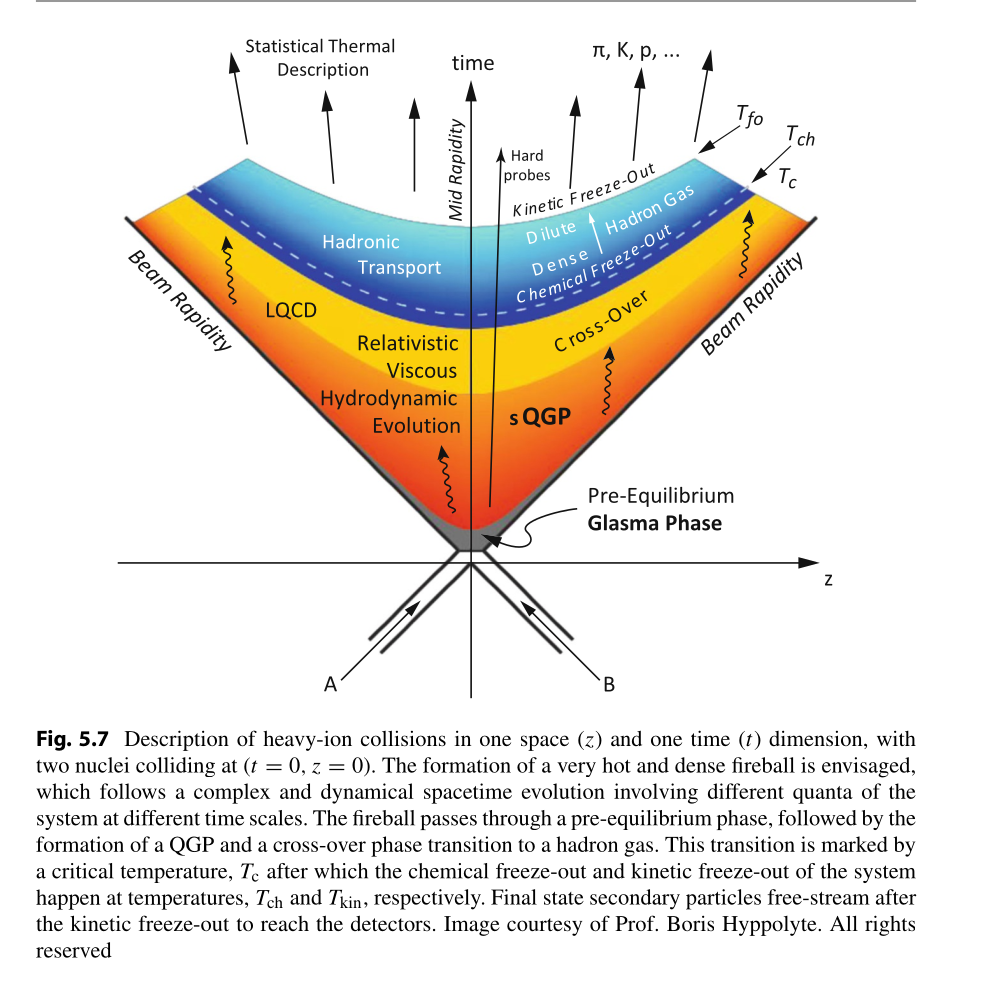
\includegraphics[width=0.95\textwidth]{plots/sahoo_fig5.7.png}
            \end{block}
        \end{column}
    \end{columns}
\end{frame}

% Slide 22: Coordinate Mappings: Light-Cone Momentum Variables
\begin{frame}{Coordinate Mappings: Light-Cone Momentum Variables}
    \begin{block}{Definitions (Sahoo pg. 119-120)}
        For ultra-relativistic collinear longitudinal processes, we define light-cone momentum variables:
        \[ p_+ = E + p_z, \quad p_- = E - p_z \]
        Which are highly advantageous since they scale simply under longitudinal boosts:
        \[ p'_+ = e^{-y_{boost}} p_+, \quad p'_- = e^{y_{boost}} p_- \]
    \end{block}
    \begin{block}{Relation to Standard Rapidity}
        Using these variables, standard momentum rapidity $y$ can be expressed as:
        \[ y = \frac{1}{2} \ln \left( \frac{p_+}{p_-} \right) \]
        In Problem 4, you verify that this formulation matches standard rapidity with exact double-precision accuracy ($|y_{lc} - y_{raw}| = 0.0$ for $2,345$ tracks).
    \end{block}
\end{frame}

% Slide 23: Coordinate Mappings: Spacetime Rapidity $\eta_s$
\begin{frame}{Coordinate Mappings: Spacetime Rapidity $\eta_s$}
    \begin{block}{Longitudinal Spacetime Scaling (Sahoo Eq. 5.44)}
        To represent the spatial coordinates $(z, t)$ of particle freezeouts in an expanding QGP medium, we define the **Spacetime Rapidity** ($\eta_s$):
        \[ \eta_s = \frac{1}{2} \ln \left( \frac{t + z}{t - z} \right) \]
        Analogously, we define the proper lifetime $\tau$:
        \[ \tau = \sqrt{t^2 - z^2} \]
    \end{block}
    \begin{block}{Bjorken Longitudinal Scaling Model}
        In ultra-relativistic collisions, spatial position and momentum become highly correlated: particles with large forward velocities end up at large forward spatial coordinates.
    \end{block}
\end{frame}

% Slide 24: Real AMPT Correlation: Spacetime vs. Momentum Rapidity
\begin{frame}{Real AMPT Correlation: Spacetime vs. Momentum Rapidity}
    \begin{columns}
        \begin{column}{0.5\textwidth}
            \begin{block}{Validation on $27,617$ Pion Tracks}
                In Problem 5 of the laboratory, you map out the $(y, \eta_s)$ scatter correlation for freezeout pions using real AMPT simulations.
                \begin{itemize}
                    \item **Linear correlation $r$:** $0.9973$
                    \item **Fitted slope:** $0.9937$
                \end{itemize}
            \end{block}
            \begin{alertblock}{Physical Conclusion}
                This near-unity slope and high correlation coefficient represent a direct validation of the **Bjorken scaling model** of relativistic longitudinal expansion!
            \end{alertblock}
        \end{column}
        \begin{column}{0.5\textwidth}
            \begin{block}{AMPT Spacetime-Momentum Correlation}
                \centering
                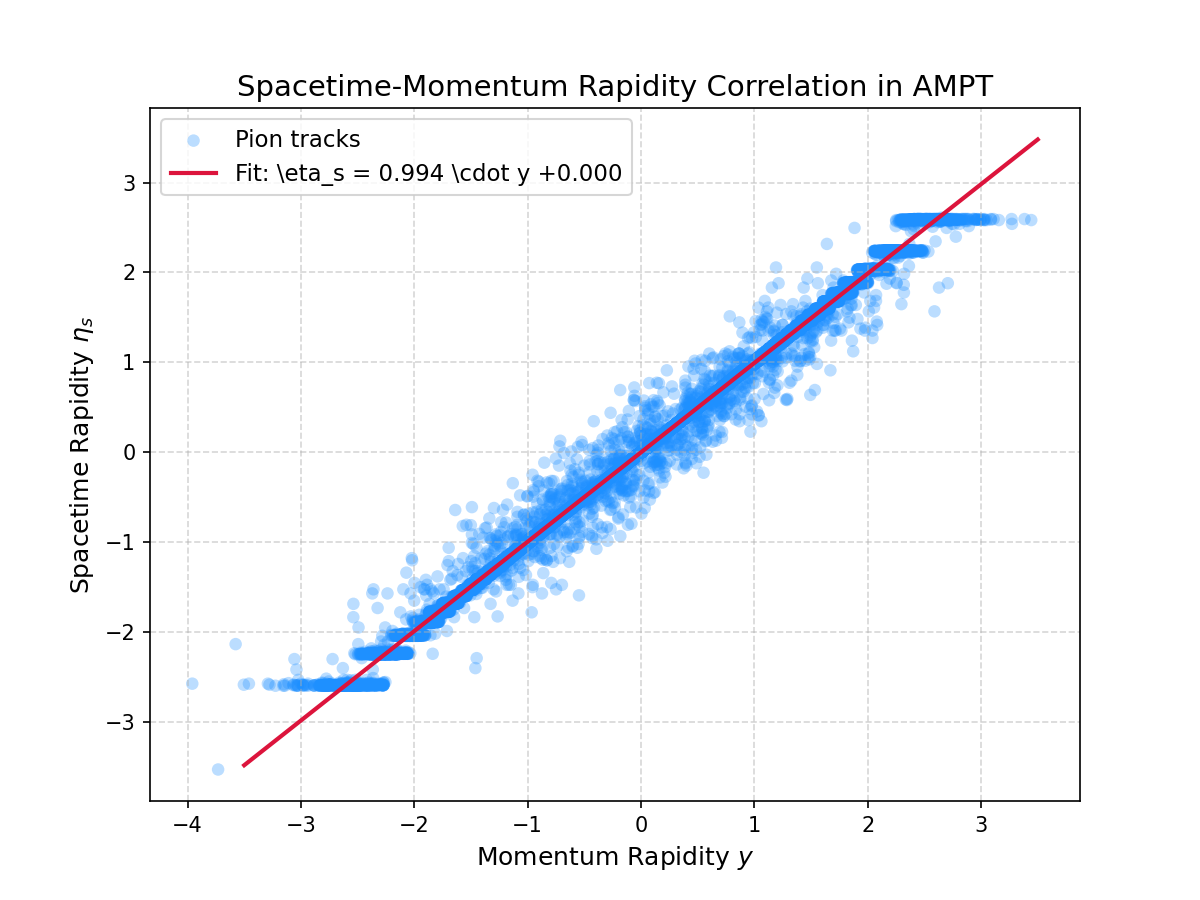
\includegraphics[width=0.85\textwidth]{exercises/day01_problem5_spacetime_correlation.png}
            \end{block}
        \end{column}
    \end{columns}
\end{frame}

% Slide 25: 3D Kinematics in Detector Planes
\begin{frame}{3D Kinematics in Detector Planes}
    \begin{block}{Transverse \& Longitudinal Decomposition (Sahoo Fig. 5.8)}
        A particle's momentum $\vec{p}$ is decomposed relative to the beam axis (Z-axis) into:
        - **Transverse Momentum ($p_T$):** curvature in TPC: $p_T = \sqrt{p_x^2 + p_y^2}$
        - **Transverse Mass ($m_T$):** $m_T = \sqrt{p_T^2 + m_0^2}$
    \end{block}
    \begin{columns}
        \begin{column}{0.5\textwidth}
            \footnotesize
            **Azimuthal Angle $\phi$ (Sahoo Eq. 5.50):**
            \[ \phi = \tan^{-1} \left( \frac{p_y}{p_x} \right) \quad [-\pi, \pi] \]
        \end{column}
        \begin{column}{0.5\textwidth}
            \footnotesize
            **Polar Angle $\theta$ (Sahoo Eq. 5.51):**
            \[ \theta = \tan^{-1} \left( \frac{p_T}{p_z} \right) \quad [0, \pi] \]
        \end{column}
    \end{columns}
\end{frame}

% Slide 26: Hyperbolic Mappings to Rapidity
\begin{frame}{Hyperbolic Mappings to Rapidity}
    \begin{block}{Standard Rapidity $y$ in term of $m_T$ (Sahoo Eq. 5.54)}
        \[ y = \frac{1}{2} \ln \left( \frac{E+p_z}{E-p_z} \right) = \ln \left( \frac{E + p_z}{m_T} \right) \]
        Which highlights the hyperbolic boost rotation of coordinates:
        \[ E = m_T \cosh y, \quad p_z = m_T \sinh y \]
    \end{block}
    \begin{block}{Pseudorapidity $\eta$ (Sahoo Eq. 5.48)}
        For highly relativistic particles ($E \gg m_0 \Rightarrow m_T \approx p_T$), standard rapidity simplifies to a purely geometric quantity called **Pseudorapidity** ($\eta$), which depends only on polar angle $\theta$:
        \[ \eta = \tanh^{-1}\left( \frac{p_z}{p} \right) = -\ln \tan \left( \frac{\theta}{2} \right) \]
    \end{block}
\end{frame}

\section{Hands-On}

% Slide 27: Summary: Day 1 Hands-On Laboratory Exercises
\begin{frame}{Summary: Day 1 Hands-On Laboratory Exercises}
    \begin{block}{Objective: Build custom Relativistic \& Coordinate Calculators}
        All exercises are framed in your Jupyter Notebook at \texttt{exercises/day01\_hands\_on.ipynb}:
    \end{block}
    \begin{enumerate}
        \footnotesize
        \item **Problem 1:** Relativistic velocity addition vs. rapidity additivity (Plot saturation).
        \item **Problem 2:** 2-body CMS energy mappings for symmetric ($p+p$, $Au+Au$) and asymmetric ($p+Pb$) systems.
        \item **Problem 3:** 3D Kinematics and coordinate decompositions (transverse variables and angles).
        \item **Problem 4:** Light-cone momentum \& rapidity on real AMPT data.
        \item **Problem 5:** Spacetime rapidity mappings and correlation checks.
    \end{enumerate}
\end{frame}

\end{document}
